% Options for packages loaded elsewhere
\PassOptionsToPackage{unicode}{hyperref}
\PassOptionsToPackage{hyphens}{url}
%
\documentclass[
]{article}
\usepackage{lmodern}
\usepackage{amssymb,amsmath}
\usepackage{ifxetex,ifluatex}
\ifnum 0\ifxetex 1\fi\ifluatex 1\fi=0 % if pdftex
  \usepackage[T1]{fontenc}
  \usepackage[utf8]{inputenc}
  \usepackage{textcomp} % provide euro and other symbols
\else % if luatex or xetex
  \usepackage{unicode-math}
  \defaultfontfeatures{Scale=MatchLowercase}
  \defaultfontfeatures[\rmfamily]{Ligatures=TeX,Scale=1}
\fi
% Use upquote if available, for straight quotes in verbatim environments
\IfFileExists{upquote.sty}{\usepackage{upquote}}{}
\IfFileExists{microtype.sty}{% use microtype if available
  \usepackage[]{microtype}
  \UseMicrotypeSet[protrusion]{basicmath} % disable protrusion for tt fonts
}{}
\makeatletter
\@ifundefined{KOMAClassName}{% if non-KOMA class
  \IfFileExists{parskip.sty}{%
    \usepackage{parskip}
  }{% else
    \setlength{\parindent}{0pt}
    \setlength{\parskip}{6pt plus 2pt minus 1pt}}
}{% if KOMA class
  \KOMAoptions{parskip=half}}
\makeatother
\usepackage{xcolor}
\IfFileExists{xurl.sty}{\usepackage{xurl}}{} % add URL line breaks if available
\IfFileExists{bookmark.sty}{\usepackage{bookmark}}{\usepackage{hyperref}}
\hypersetup{
  pdftitle={covid tree analysis},
  hidelinks,
  pdfcreator={LaTeX via pandoc}}
\urlstyle{same} % disable monospaced font for URLs
\usepackage[margin=1in]{geometry}
\usepackage{color}
\usepackage{fancyvrb}
\newcommand{\VerbBar}{|}
\newcommand{\VERB}{\Verb[commandchars=\\\{\}]}
\DefineVerbatimEnvironment{Highlighting}{Verbatim}{commandchars=\\\{\}}
% Add ',fontsize=\small' for more characters per line
\usepackage{framed}
\definecolor{shadecolor}{RGB}{248,248,248}
\newenvironment{Shaded}{\begin{snugshade}}{\end{snugshade}}
\newcommand{\AlertTok}[1]{\textcolor[rgb]{0.94,0.16,0.16}{#1}}
\newcommand{\AnnotationTok}[1]{\textcolor[rgb]{0.56,0.35,0.01}{\textbf{\textit{#1}}}}
\newcommand{\AttributeTok}[1]{\textcolor[rgb]{0.77,0.63,0.00}{#1}}
\newcommand{\BaseNTok}[1]{\textcolor[rgb]{0.00,0.00,0.81}{#1}}
\newcommand{\BuiltInTok}[1]{#1}
\newcommand{\CharTok}[1]{\textcolor[rgb]{0.31,0.60,0.02}{#1}}
\newcommand{\CommentTok}[1]{\textcolor[rgb]{0.56,0.35,0.01}{\textit{#1}}}
\newcommand{\CommentVarTok}[1]{\textcolor[rgb]{0.56,0.35,0.01}{\textbf{\textit{#1}}}}
\newcommand{\ConstantTok}[1]{\textcolor[rgb]{0.00,0.00,0.00}{#1}}
\newcommand{\ControlFlowTok}[1]{\textcolor[rgb]{0.13,0.29,0.53}{\textbf{#1}}}
\newcommand{\DataTypeTok}[1]{\textcolor[rgb]{0.13,0.29,0.53}{#1}}
\newcommand{\DecValTok}[1]{\textcolor[rgb]{0.00,0.00,0.81}{#1}}
\newcommand{\DocumentationTok}[1]{\textcolor[rgb]{0.56,0.35,0.01}{\textbf{\textit{#1}}}}
\newcommand{\ErrorTok}[1]{\textcolor[rgb]{0.64,0.00,0.00}{\textbf{#1}}}
\newcommand{\ExtensionTok}[1]{#1}
\newcommand{\FloatTok}[1]{\textcolor[rgb]{0.00,0.00,0.81}{#1}}
\newcommand{\FunctionTok}[1]{\textcolor[rgb]{0.00,0.00,0.00}{#1}}
\newcommand{\ImportTok}[1]{#1}
\newcommand{\InformationTok}[1]{\textcolor[rgb]{0.56,0.35,0.01}{\textbf{\textit{#1}}}}
\newcommand{\KeywordTok}[1]{\textcolor[rgb]{0.13,0.29,0.53}{\textbf{#1}}}
\newcommand{\NormalTok}[1]{#1}
\newcommand{\OperatorTok}[1]{\textcolor[rgb]{0.81,0.36,0.00}{\textbf{#1}}}
\newcommand{\OtherTok}[1]{\textcolor[rgb]{0.56,0.35,0.01}{#1}}
\newcommand{\PreprocessorTok}[1]{\textcolor[rgb]{0.56,0.35,0.01}{\textit{#1}}}
\newcommand{\RegionMarkerTok}[1]{#1}
\newcommand{\SpecialCharTok}[1]{\textcolor[rgb]{0.00,0.00,0.00}{#1}}
\newcommand{\SpecialStringTok}[1]{\textcolor[rgb]{0.31,0.60,0.02}{#1}}
\newcommand{\StringTok}[1]{\textcolor[rgb]{0.31,0.60,0.02}{#1}}
\newcommand{\VariableTok}[1]{\textcolor[rgb]{0.00,0.00,0.00}{#1}}
\newcommand{\VerbatimStringTok}[1]{\textcolor[rgb]{0.31,0.60,0.02}{#1}}
\newcommand{\WarningTok}[1]{\textcolor[rgb]{0.56,0.35,0.01}{\textbf{\textit{#1}}}}
\usepackage{graphicx,grffile}
\makeatletter
\def\maxwidth{\ifdim\Gin@nat@width>\linewidth\linewidth\else\Gin@nat@width\fi}
\def\maxheight{\ifdim\Gin@nat@height>\textheight\textheight\else\Gin@nat@height\fi}
\makeatother
% Scale images if necessary, so that they will not overflow the page
% margins by default, and it is still possible to overwrite the defaults
% using explicit options in \includegraphics[width, height, ...]{}
\setkeys{Gin}{width=\maxwidth,height=\maxheight,keepaspectratio}
% Set default figure placement to htbp
\makeatletter
\def\fps@figure{htbp}
\makeatother
\setlength{\emergencystretch}{3em} % prevent overfull lines
\providecommand{\tightlist}{%
  \setlength{\itemsep}{0pt}\setlength{\parskip}{0pt}}
\setcounter{secnumdepth}{-\maxdimen} % remove section numbering
\usepackage{booktabs}
\usepackage{longtable}
\usepackage{array}
\usepackage{multirow}
\usepackage{wrapfig}
\usepackage{float}
\usepackage{colortbl}
\usepackage{pdflscape}
\usepackage{tabu}
\usepackage{threeparttable}
\usepackage{threeparttablex}
\usepackage[normalem]{ulem}
\usepackage{makecell}
\usepackage{xcolor}

\title{covid tree analysis}
\author{}
\date{\vspace{-2.5em}}

\begin{document}
\maketitle

\hypertarget{cross-sectional-analysis-of-covid-19-spread-in-us-counties}{%
\section{Cross sectional Analysis of Covid-19 Spread in US
Counties}\label{cross-sectional-analysis-of-covid-19-spread-in-us-counties}}

\hypertarget{introduction}{%
\section{Introduction}\label{introduction}}

Covid-19 or corona virus started its spread from China at the end of
Year 2020. By February 2020, cases start to appear in the United States
and spread rapidly across all the states. The growth in the number of
cases has been exponential like any other case of infectious disease.
Scientists and researchers around the world are actively looking at the
data to understand this virus. In uncertain times like these, it is
important to know the factors that affect the spread of this virus to
make plausible predictions about the future.

Since the first case of covid-19 was discovered in the US in Snohomish
county in the Washington State, the virus has now spread to other places
and in some cities like New York and Chicago, the spread has been
faster, making them new hotspots for the virus even though cities like
Seattle \& Los Angeles reported their first cases before these cities. A
simple line graphs for some counties that saw their first case of
infection around the same time shows the difference in the rate of virus
spread.

\begin{figure}
\centering
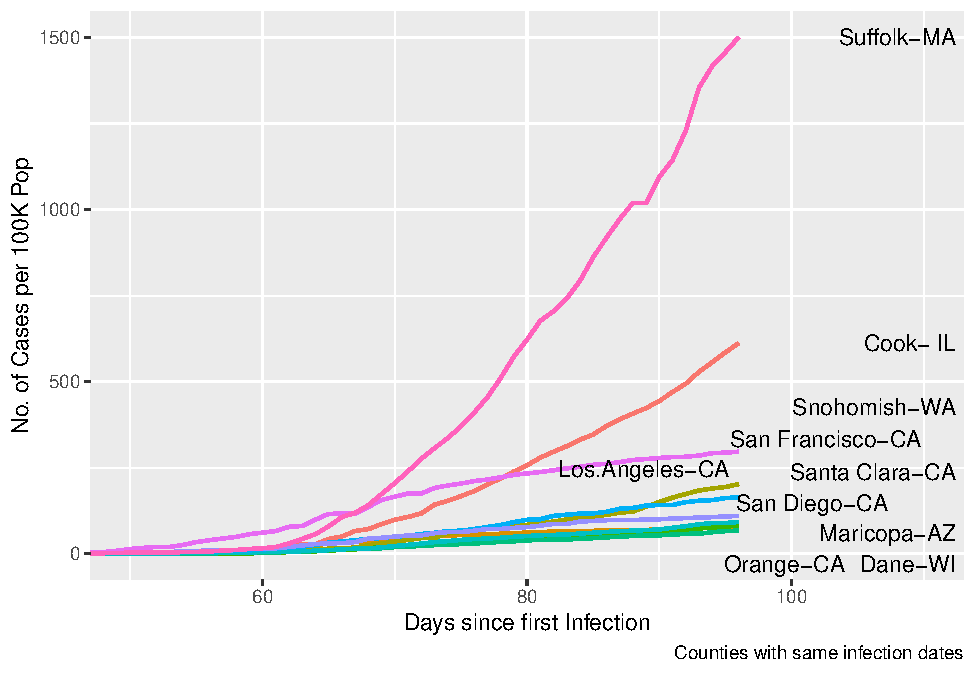
\includegraphics{covid_tree_analysis_files/figure-latex/unnamed-chunk-2-1.pdf}
\caption{Trend Line Graph for Counties}
\end{figure}

This poses a question that; what are the different factors that are
leading to differences in the pace of covid-19 spread across US
counties? Can a cross sectional comparison of these counties help us
identify any socio-economic or geographical feature that has any effect
on virus spread and can we use these features to predict the number of
infections for other counties that are behind in trend. We carry out a
cross sectional analysis of counties and their features in comparison to
the number of covid-19 cases reported by using statistical and data
mining tools. The purpose of the report is to identify any trend or
characteristics of counties that are connected to the pace of virus
spread.

\hypertarget{data}{%
\section{Data}\label{data}}

\begin{itemize}
\tightlist
\item
  \textbf{Cases \& Deaths:} We collect the data of total number of
  covid-19 infection cases and deaths at county level as on April 30,
  2010. The data has been obtained from NYTimes Github repository. We
  selected 1462 counties which had non-zero number of deaths reported.
  This was done because ACS data was only available for counties that
  have any death reported for covid-19.We divided the total number of
  cases by population to have cases per hundred thousand of population.
  This gives a good comparison of cases across counties with different
  population size. From now on we will refer to cases as cases per
  hundred thousand of population. The density graph shows that a lot of
  counties have lower number of cases and a very skewed distribution of
  cases.
\end{itemize}

\begin{figure}
\centering
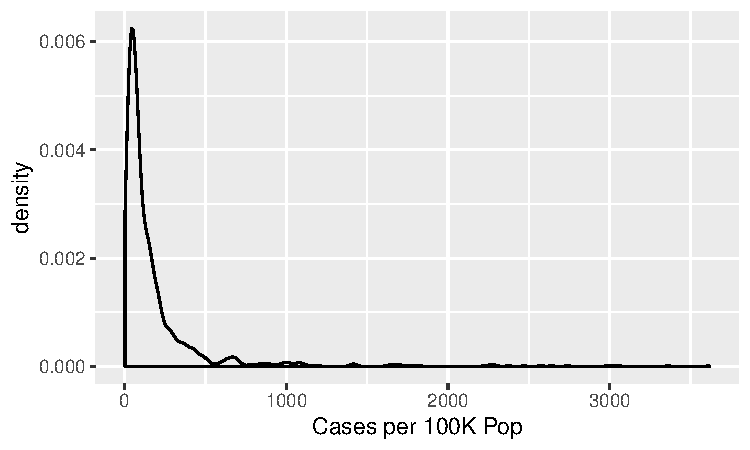
\includegraphics{covid_tree_analysis_files/figure-latex/unnamed-chunk-3-1.pdf}
\caption{Density Graph for Number of Cases}
\end{figure}

\begin{itemize}
\tightlist
\item
  \textbf{Days since first Case:} We calculated the total number of days
  since 1st infection for all counties as on April 30, 2020. This
  variable measures the time period for spread of virus. A scatter plot
  of days since first infection and number of cases per 100 thousand
  people shows that there is a general exponential trend but some
  counties have been able to keep their number of cases down even though
  the got the virus before other counties.
\end{itemize}

\begin{Shaded}
\begin{Highlighting}[]
\KeywordTok{ggplot}\NormalTok{(covid, }\DataTypeTok{mapping =} \KeywordTok{aes}\NormalTok{(days_since_first_infection1,cases1))}\OperatorTok{+}\KeywordTok{geom_point}\NormalTok{()}\OperatorTok{+}\KeywordTok{labs}\NormalTok{(}\DataTypeTok{title=} \StringTok{"Scatter Plot of Time and Cases"}\NormalTok{,}\DataTypeTok{y=}\StringTok{"Cases per 100K Pop"}\NormalTok{)}
\end{Highlighting}
\end{Shaded}

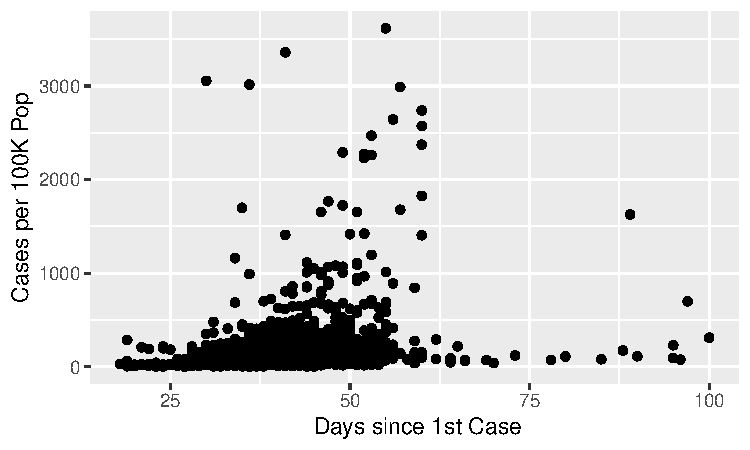
\includegraphics{covid_tree_analysis_files/figure-latex/unnamed-chunk-4-1.pdf}

\begin{itemize}
\tightlist
\item
  \textbf{Days since Stay at home orders:} Similarly, we calculated
  number of days since stay at home orders were issued by State and
  County authorities as on April 30, 2020. This gives us the time period
  for interventions taken by authorities. Along with this we also
  obtained Google's movement analytics for each county which gives a
  percentage decline in people's movement from the baseline average.
\item
  \textbf{Socio-Economic Variables:} We obtained socio economic
  variables on the population of counties from American Community Survey
  reports. Main variables include: Unemployment rate, \% of White, \% of
  Households in Poverty, \% of population employed in different
  industries, median income and \% of population with a bachelor's
  degree.\\
\item
  \textbf{Demographic Variables:} \% of male, \% of age between 18 and
  64, \% of White, Median age, \% of total households as family etc. The
  complete list is attached in the appendix.
\item
  \textbf{Geographical variables:} We obtained variables like population
  density, average of last 8 years highest summer temperature and
  humidity rate. We wanted to obtain the recent monthly averages for
  counties but could not find the latest data, so we used these
  variables.
\end{itemize}

There were many socio-economic variables that were very highly
correlated, so we dropped some variables and finalized 30 variables for
this analysis. The complete list of these variables is provided in the
appendix.

\textbf{Note} :Before we start with our analysis, it is important that
we acknowledge that number of cases reported depends heavily on the
number of tests conducted. Unfortunately, testing policy has not been
uniformed across US and that can lead to a measurement error in cases.
Secondly, there are reports that the given time frame for start of
covid-19 is not accurate and it is presumed that covid-19 reached many
major cities of the US way before the first case was reported.

However, due to data limitation, we must assume that the official
reporting of cases represents somewhat actual position for the start of
virus infection. For testing, we tried to get data on total tests
conducted on county level but only find the data at state level. So, we
calculated total tests conducted per hundred thousand people for each
state and then use it for each county in respective state. This is not
perfect, but we are assuming that the rate of testing is uniform across
counties in each state and will help in differentiating counties of
different states based on testing rates.

\hypertarget{methods}{%
\section{Methods}\label{methods}}

\hypertarget{principal-component-analysis}{%
\subsection{Principal Component
Analysis}\label{principal-component-analysis}}

We use principal component analysis to see if we can look at the
variations in the counties and evaluate if those variations are related
to number of cases in these counties. After scaling the data, we see
that 90\% of variation in 30 explanatory variables can be explained by
16 principal components, pointing towards correlation between these
variables.

The biplot of main variables that contribute to variance is first two
PCs shows that PC1 captures variation in population density, time since
first case, proportion of population between 18 and 64 and change in the
movement of people to their workplaces.

\begin{Shaded}
\begin{Highlighting}[]
\KeywordTok{library}\NormalTok{(factoextra)}
\end{Highlighting}
\end{Shaded}

\begin{verbatim}
## Warning: package 'factoextra' was built under R version 3.6.3
\end{verbatim}

\begin{verbatim}
## Welcome! Want to learn more? See two factoextra-related books at https://goo.gl/ve3WBa
\end{verbatim}

\begin{Shaded}
\begin{Highlighting}[]
\NormalTok{covid =}\StringTok{ }\KeywordTok{read.csv}\NormalTok{(}\StringTok{"covid2zargham.csv"}\NormalTok{)}
\NormalTok{X=}\StringTok{ }\NormalTok{covid[,}\OperatorTok{-}\KeywordTok{c}\NormalTok{(}\DecValTok{1}\OperatorTok{:}\DecValTok{5}\NormalTok{, }\DecValTok{35}\NormalTok{,}\DecValTok{37}\NormalTok{)]}
\NormalTok{PCA =}\StringTok{ }\KeywordTok{prcomp}\NormalTok{(X, }\DataTypeTok{scale. =} \OtherTok{TRUE}\NormalTok{)}
\KeywordTok{fviz_pca_var}\NormalTok{(PCA, }\DataTypeTok{col.var=}\StringTok{"contrib"}\NormalTok{,}
             \DataTypeTok{gradient.cols =} \KeywordTok{c}\NormalTok{(}\StringTok{"#00AFBB"}\NormalTok{, }\StringTok{"#E7B800"}\NormalTok{, }\StringTok{"#FC4E07"}\NormalTok{),}\DataTypeTok{select.var =} \KeywordTok{list}\NormalTok{(}\DataTypeTok{contrib=}\DecValTok{12}\NormalTok{),}
             \DataTypeTok{repel =} \OtherTok{TRUE}\NormalTok{, }\DataTypeTok{title =} \StringTok{"Variables Contribution in first two PCAs "}\NormalTok{ )}
\end{Highlighting}
\end{Shaded}

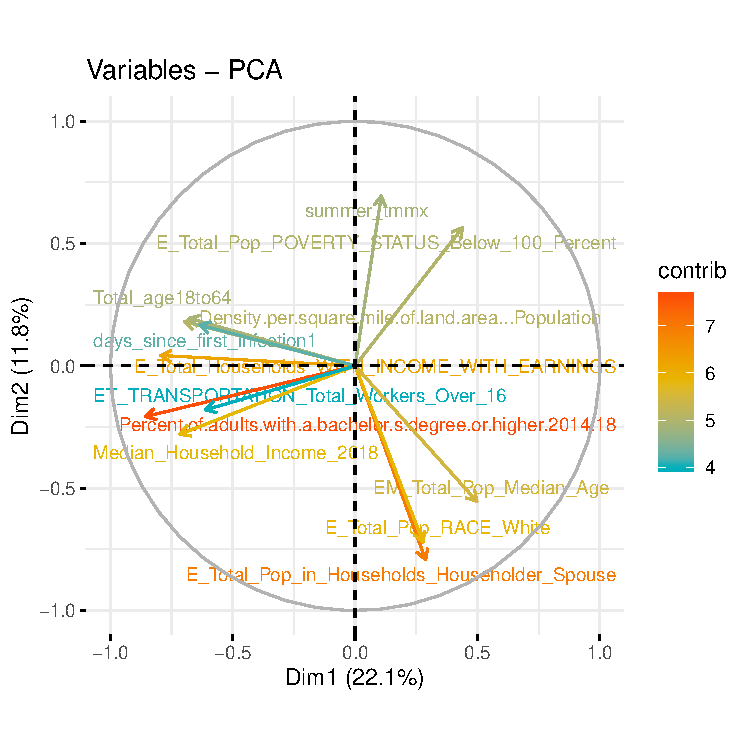
\includegraphics{covid_tree_analysis_files/figure-latex/unnamed-chunk-5-1.pdf}

\begin{Shaded}
\begin{Highlighting}[]
\NormalTok{scores =}\StringTok{ }\NormalTok{PCA}\OperatorTok{$}\NormalTok{x}
\NormalTok{scores=}\StringTok{ }\KeywordTok{cbind}\NormalTok{(covid}\OperatorTok{$}\NormalTok{cases1, scores)}
\NormalTok{scores =}\StringTok{ }\KeywordTok{as.data.frame}\NormalTok{(scores)}
\KeywordTok{qplot}\NormalTok{(PC1,PC2, }\DataTypeTok{data=}\NormalTok{scores, }\DataTypeTok{color=}\NormalTok{ V1)}\OperatorTok{+}\KeywordTok{scale_color_gradient}\NormalTok{(}\DataTypeTok{low =} \StringTok{"grey"}\NormalTok{, }\DataTypeTok{high=} \StringTok{'red'}\NormalTok{)}\OperatorTok{+}\KeywordTok{ggtitle}\NormalTok{(}\StringTok{"Cluster Plot of Cases and First two Principal Components"}\NormalTok{)}\OperatorTok{+}\KeywordTok{labs}\NormalTok{(}\DataTypeTok{color =} \StringTok{"Cases per 100K Pop"}\NormalTok{)}
\end{Highlighting}
\end{Shaded}

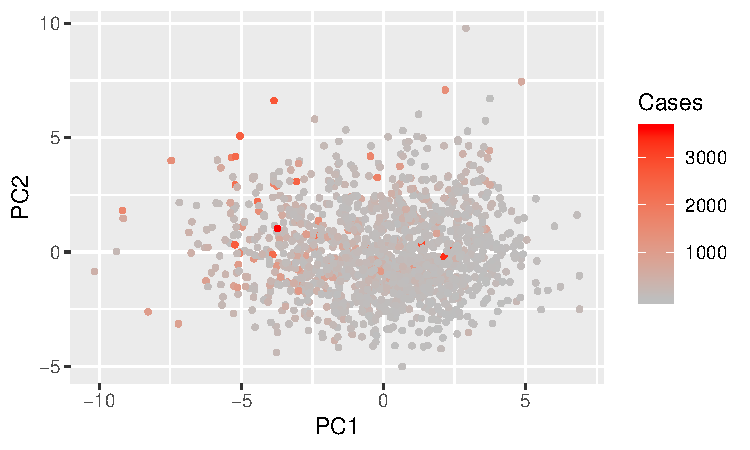
\includegraphics{covid_tree_analysis_files/figure-latex/unnamed-chunk-6-1.pdf}

Plotting the scatter plot with first two components with color scaling
the number of cases, we see that there is no specific clustering of high
cases counties but generally, we see that there are more red points in
the upper left quadrant of the graph. Which means that variables
mentioned above are correlated with higher number of covid-19 cases in
counties. Similarly, lower right quadrant has less number of high case
counties and from the biplot we saw that this is associated with higher
proportion of white population, higher median age and higher proportion
of spouse households in total households. Interestingly, we cannot say
much about the effect of temperature on virus spread but there does
seems to be a slight negative correlation between temperature and virus
spread.

\hypertarget{negative-binomial-logistic-model}{%
\subsection{Negative Binomial Logistic
Model}\label{negative-binomial-logistic-model}}

Since our outcome is count of cases with overdispersion, we fit a
negative binomial logistic model on our data. As we have only those
counties that reported the any cases, we use zero truncated negative
binomial logistic model. This model has been used by
\href{https://www.medrxiv.org/node/78162.external-links.html}{Wu,Nethery,Sabath
(2020)} in their study of exposure to air pollution and its effect on
covid death rate in US counties. We include all the explanatory
variables in our model to which of them are correalted with cases count.
The summary of the model is provided in the appendix.

We can clearly see that infection start date is positively correlated
with the log count of cases. Along with it, stay at home orders are
linked negatively to cases growth which is also theoretically correct.
Another important variable is population density per square mile area
which means that congested counties see higher number of cases. Counties
with higher percentage of educated people and people with race as white
also observe lower cases. Higher proportion of people employed in
educational and health services and lower proportion of people in arts,
recreational, accommodation and public administration industries are
correlated with higher cases of virus. The signs for these co-efficient
are consistent with our PCA analysis.\\
We have a problem of small sample and it would have been better if the
sample size could have been bigger. We have Hauck-Donner effect in two
variables: \% of population age 18 to 64 and
E\_Total\_Households\_TYPE\_Family. The co-efficient magnitude cannot be
considered as casual effect. However, the signs of co-efficient points
towards some plausible correlation between number of cases and different
variables. To check the predictive power of our model, we do 300 test/
train splits of our sample and run the model. We get a RMSE of around
240 cases per hundred thousand people. Plotting the predicted values
against the actual values, we see that the model on average
underpredicts the number of cases for counties with high number of cases
and overpredicts for counties with lower number of cases. Overall, we do
not think this model does a good job at prediction.

\begin{verbatim}
## [1] 242.3946
\end{verbatim}

\begin{Shaded}
\begin{Highlighting}[]
\NormalTok{yhat1 =}\StringTok{ }\KeywordTok{predict}\NormalTok{(m12, }\DataTypeTok{type =} \StringTok{'response'}\NormalTok{)}
\NormalTok{modelfit1=}\StringTok{ }\KeywordTok{as.data.frame}\NormalTok{(}\KeywordTok{cbind}\NormalTok{(yhat1, covid}\OperatorTok{$}\NormalTok{cases1))}

\NormalTok{b1=}\KeywordTok{ggplot}\NormalTok{(modelfit1, }\DataTypeTok{mapping =} \KeywordTok{aes}\NormalTok{(V2, V1))}\OperatorTok{+}\KeywordTok{geom_point}\NormalTok{()}\OperatorTok{+}\KeywordTok{geom_abline}\NormalTok{(}\DataTypeTok{slope =} \DecValTok{1}\NormalTok{,}\DataTypeTok{intercept =} \DecValTok{0}\NormalTok{)}\OperatorTok{+}\StringTok{ }\KeywordTok{labs}\NormalTok{(}\DataTypeTok{x=}\StringTok{"Actual"}\NormalTok{, }\DataTypeTok{y=} \StringTok{"Predicted"}\NormalTok{, }\DataTypeTok{title =} \StringTok{"Cases per 100K Pop"}\NormalTok{)}\OperatorTok{+}\KeywordTok{theme}\NormalTok{(}\DataTypeTok{plot.title =} \KeywordTok{element_text}\NormalTok{(}\DataTypeTok{size =}\DecValTok{10}\NormalTok{))}

\NormalTok{b2=}\StringTok{ }\KeywordTok{ggplot}\NormalTok{(modelfit1, }\DataTypeTok{mapping =} \KeywordTok{aes}\NormalTok{(V2, V1))}\OperatorTok{+}\KeywordTok{geom_point}\NormalTok{()}\OperatorTok{+}\KeywordTok{geom_abline}\NormalTok{(}\DataTypeTok{slope =} \DecValTok{1}\NormalTok{,}\DataTypeTok{intercept =} \DecValTok{0}\NormalTok{)}\OperatorTok{+}\StringTok{ }\KeywordTok{labs}\NormalTok{(}\DataTypeTok{x=}\StringTok{"Actual"}\NormalTok{, }\DataTypeTok{y=} \StringTok{"Predicted"}\NormalTok{, }\DataTypeTok{title =} \StringTok{"Cases per 100K Pop - Low Values"}\NormalTok{)}\OperatorTok{+}\KeywordTok{coord_cartesian}\NormalTok{(}\DataTypeTok{xlim =} \KeywordTok{c}\NormalTok{(}\DecValTok{0}\NormalTok{, }\DecValTok{1000} \OperatorTok{+}\StringTok{ }\DecValTok{10}\NormalTok{))}\OperatorTok{+}\KeywordTok{theme}\NormalTok{(}\DataTypeTok{plot.title =} \KeywordTok{element_text}\NormalTok{(}\DataTypeTok{size =}\DecValTok{10}\NormalTok{))}

\KeywordTok{grid.arrange}\NormalTok{(b1,b2, }\DataTypeTok{widths=}\KeywordTok{c}\NormalTok{(}\FloatTok{0.5}\NormalTok{, }\FloatTok{0.5}\NormalTok{) , }\DataTypeTok{heights=}\KeywordTok{c}\NormalTok{(}\FloatTok{0.7}\NormalTok{, }\FloatTok{0.7}\NormalTok{),}\DataTypeTok{ncol =} \DecValTok{2}\NormalTok{)}
\end{Highlighting}
\end{Shaded}

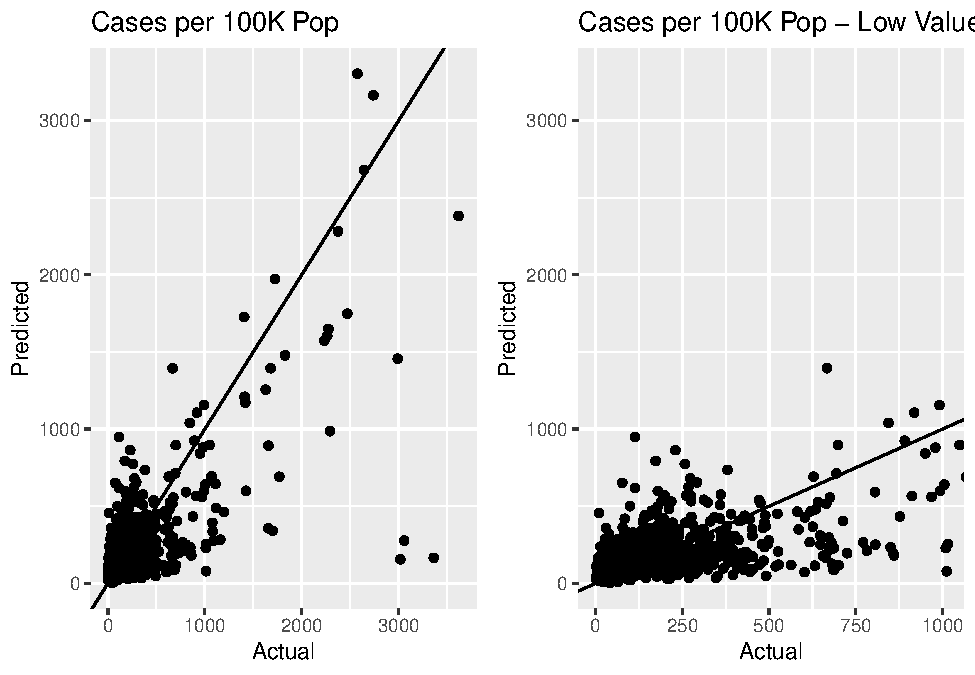
\includegraphics{covid_tree_analysis_files/figure-latex/unnamed-chunk-9-1.pdf}

We try the same model with actual number of cases rather than number of
cases per hundred thousand people and include log of population in the
model to control for community size. The RMSE of 300 test and train
split comes out to be around 1500 and the prediction graph is more
balanced as compared to the model with cases per hundred thousand
population. Therefore, we prefer using total number of cases in the
model for prediction purpose.

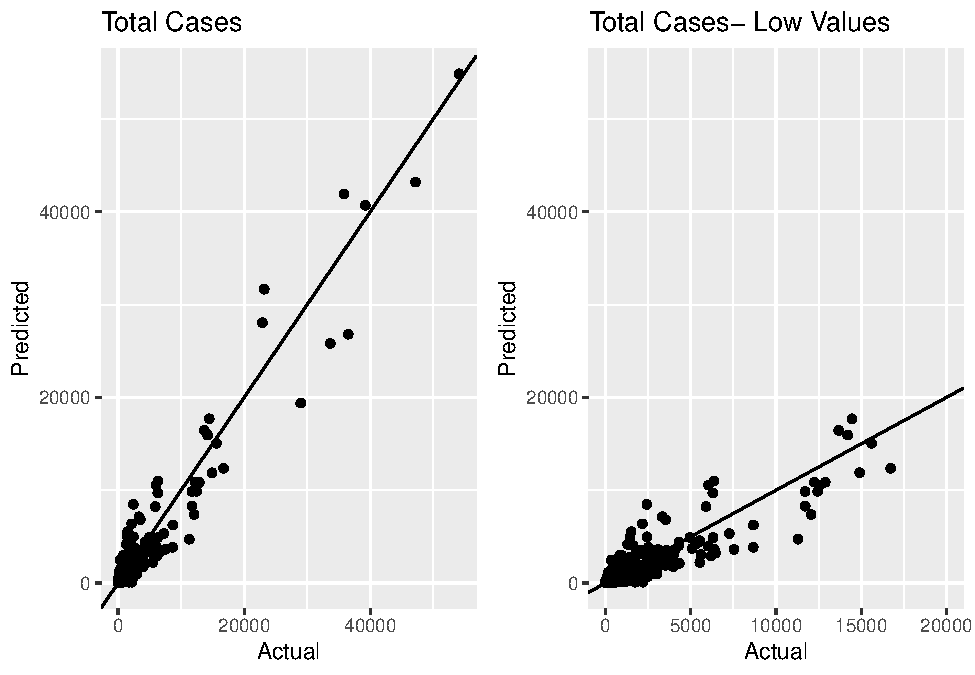
\includegraphics{covid_tree_analysis_files/figure-latex/unnamed-chunk-11-1.pdf}

\hypertarget{analysis-using-random-forest-and-boosting-trees}{%
\subsection{Analysis using Random Forest and Boosting
Trees}\label{analysis-using-random-forest-and-boosting-trees}}

In this section we perform an anlysis over the county level data of
Covid-19 reports. We know that the tree models are characterized to be
flexible fitters that can capture non-linearity and interactions between
the variables. Tree models also are useful when we have information in
different magnitudes as this case, where we have variables that are
values while others are proportions. Specifically, we will work with
with a Random Forest model and a Boosting Tree mode. The first, model
mainly fit many large trees to bootstrap-resampled versions of the
training data by relevance, while the second fits several trees to
reweighted versions of the training dataset and then classifies by
weighted majority relevance.

Our goal in this section will be fittin models on cases per 100k
population. As in the previous section, our data set includes a set of
socieconomic, demographic and geographical variables for many US states.
The data set includes information about the Covid crisis such as tests
per 100k population and policies issued to fight the pandemic. By the
use of this sort of models we can get information about variable
relevance, that can shed light about what variables make more likely the
presence of the disease in a community and to improve the understanding
of this pandemic. To run our models, we first splitted our sample in a
training and test subsamples in order to confirm the model performance.
After this, We created 1000 trees by random forest including a minimum
of 5 features per bucket, and later we compute the out of sample RMSE.

Table XX summarizes the variable importance information derived from the
random forest model (RF). We can notice that as expected the population
density per square mile plays an importante role as expected. It suggest
that Counties more dense must expect a higher number of people infected,
as happened in New York state. The RF model also suggets that the number
of test performed in county matters, this goes in the direction of
people that support the lower initial of reported cases in the US was
due to the lack of testing. The RF model shows that the variable that
measures the decrease in number of people at work places is relevant,
which may suggest two things, one that places that started the lockdown
earlier could have more cases or the lockdown did stop the virus
expansion, since variable importance here does not gives us the impact
sign. From the variable importance table we can also see covariates
related with the population that have had more exposition the the virus,
such as occupation. We can see that the proportion of people working at
food services in a county explains the number of cases, which make sense
since this sort of jobs are likely to have contact with many people,
increasing the probability to get sick. As mentioned, we fit a Boosting
Tree(BT) that allows us to validate the results of the RF model. The BT
model generate a variable importance output as well, the result in this
case are close with those released by the RF and are summarized in table
XX.

\begin{verbatim}
## Warning in rug(quantile(xv, seq(0.1, 0.9, by = 0.1)), side = 1): some values
## will be clipped

## Warning in rug(quantile(xv, seq(0.1, 0.9, by = 0.1)), side = 1): some values
## will be clipped

## Warning in rug(quantile(xv, seq(0.1, 0.9, by = 0.1)), side = 1): some values
## will be clipped

## Warning in rug(quantile(xv, seq(0.1, 0.9, by = 0.1)), side = 1): some values
## will be clipped
\end{verbatim}

\begin{figure}
\centering
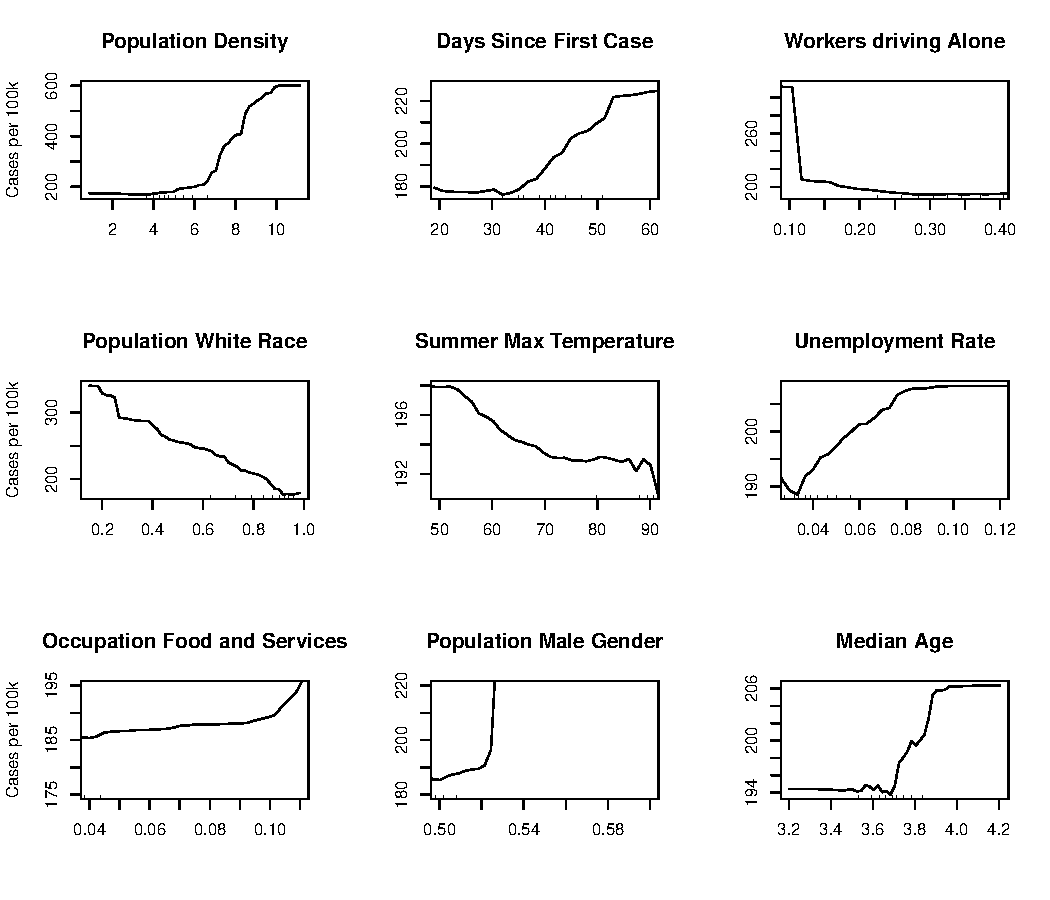
\includegraphics{covid_tree_analysis_files/figure-latex/fig1-1.pdf}
\caption{Partial Dependence From Random Forest Model}
\end{figure}

From Random Forest model and Boosting Trees we have the posibility to
generate partial dependence functions. This functions show the marginal
effect of one feature on the predicted outcome of our model. A partial
dependence function can be represented as:




Where \(x_i\) are the variables for which we are computing the function
and matrix X the other variables used in the model \(\hat{g}\). Then,
the partial function tell us for a given value of covariate \(i\) what
the average marginal effect on the prediction is. Then by the
calculation of the partial depence functions we can look for the effect
of the County level features over the number of Covid cases per 100k.
Figure \ref{fig:fig1} shows the partial depence function derived of the
RF for some features we found intuitive, for example we can observe the
can confirm the positive relation of population density over number of
cases. We also can evaluate the effect of a socioeconomic variable such
as poverty level, specifically we can see that an increase of poverty
level has a positive impact over number of cases. In the case of
proportion of population being white has a negative effect on number of
cases. This finding goes in line with the last reports of New York State
that suggest that the most affected ethnicity or race are Hispanic and
Black. It is also interesting to see how warmer summer temperatures have
a negative effect over Covid cases. Finally, we can see how a higher
median age has a positive effect and more people driving alone to work
has a negative one.

Regarding to the predictive performance of the models, we got an out of
sample RMSE of 203.1140734 for the RF model and 236.0619057 for the BT.
This values sugget that these models are reasonable tools for prediction
even tough they do not outperform the result of the Negative Binomial
model on cases per 100k.

\end{document}
